

\chapter{Experimentos con ataques adversarios} % Main chapter title

\label{Experimentos} % Change X to a consecutive number; for referencing this chapter elsewhere, use \ref{ChapterX}

%----------------------------------------------------------------------------------------
%	SECTION 1
%----------------------------------------------------------------------------------------

En esta sección se presentan distintos experimentos en donde se implementan y evalúan ataques adversarios. Se implementaron en Python desde un notebook generado en Jupyter. También se utilizaron los marcos de trabajos Keras y Tensorflow ejecutando procesos en la GPU a través de CUDA (drivers de tarjeta gráfica Nvidia).


\section{Ambiente de trabajo}
Esta práctica fue realizada en las siguientes condiciones de hardware y software:
\begin{itemize}
    \item Software
        \begin{itemize}
            \item Sistema Operativo: Ubuntu 20.04
            \item nvcc: NVIDIA (R) Cuda compiler driver
            \item Librerías: Keras (Tensorflow como backend)
        \end{itemize}
    \item Hardware
        \begin{itemize}
            \item Procesador: i7-9750H, 2.60 GHz, 6 nucleos, 12 MB Cache
            \item GPU: Nvidia GTX 1650 MAX Q, 4GB
            \item RAM: 32 GB DDR4
        \end{itemize}
\end{itemize}


\section{Repositorio}
El código fuente de estos experimentos se encuentra publicado en Github, y está desarrollado en lenguaje Python, creado en notebooks de Júpiter.
La URL del repositorio es la siguiente:\\ \url{https://github.com/rodrigo-orellana/Seguridad-en-redes-neuronales-artificiales}



\section{Ataques adversarios en fashion MNIST: Transferibilidad}
Este experimento se llevó a cabo con la intención de comprobar la transferibilidad \parencite{r4} de ejemplos adversarios de un modelo a otro cuando ambos modelos poseen el mismo tipo de clasificación. Se diseñó bajo los supuestos siguientes:
\begin{itemize}
    \item El atacante posee acceso solo a ingresar imágenes en la entrada y observar el resultado de la clasificación del modelo objetivo de su ataque.
    \item El atacante tiene acceso al conjunto de datos utilizado en el entrenamiento del modelo objetivo del ataque.
    \item El atacante crea su propio modelo sustituto, en cual posee una arquitectura y parámetros distintos al del modelo objetivo del ataque, pero es entrenado con el mismo conjunto de datos.
    \item El atacante crea ejemplos adversarios utilizando las gradientes descendientes del modelo sustituto y haciendo uso de imágenes de prueba del conjunto de datos.
    \item El atacante ejecuta su ataque con los ejemplos adversarios creados en su modelo sustituto.
\end{itemize}


\subsection{Conjunto de datos fashion MNIST}
Fashion-MNIST es un conjunto de datos de imágenes de los artículos de la tienda de moda Zalando, que consta de un conjunto de entrenamiento de 60.000 ejemplos y un conjunto de validación de 10.000 ejemplos. Cada ejemplo es una imagen en escala de grises de 28x28, asociada con una etiqueta de 10 clases que se muestran en la figura~\ref{fig:36}.

\begin{figure}[!h]
\centering
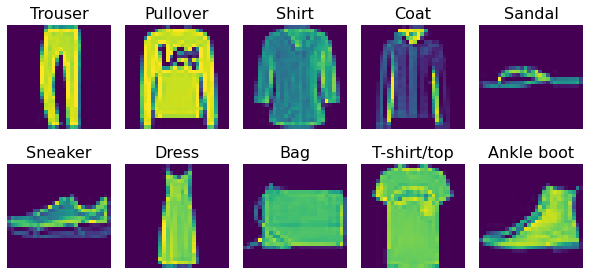
\includegraphics[scale = 0.92]{Figures/figura_36.PNG}
\decoRule
\caption[Redes generativas con adversario (GAN) como defensas]{Muestra de las 10 clases del conjunto de datos fashion-MNIST.}
\label{fig:36}
\end{figure}

\subsection{Modelo sustituto}
Se creó un modelo que llamaremos sustituto, el cual tiene como propósito generar ejemplos adversarios a ser utilizados a otros modelos que presentaremos a continuación en modalidad de caja negra. La red utilizada es una CNN simple, su arquitectura se observa en la figura~\ref{fig:model}.

\begin{figure}[!h]
\centering
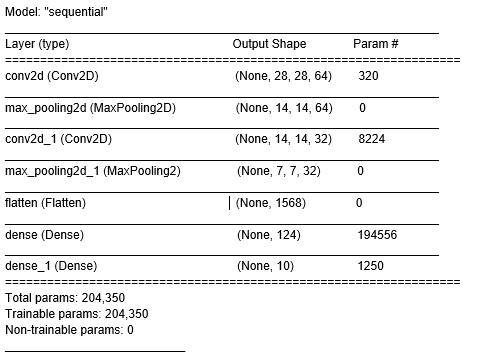
\includegraphics{Figures/model_F_MNIST.PNG}
\decoRule
\caption[Arquitectura modelo sustituto fashion-MNIST]{Arquitectura modelo sustituto}
\label{fig:model}
\end{figure}

Para validar que los modelos creados en el experimento funcionan correctamente presentamos en la figura~\ref{fig:37} una gráfica de exactitud de los modelos validados en los datos de validación. El modelo 01 corresponde al modelo sustituto, mientras que los modelos del 02 al 06 son las víctimas. La exactitud de los modelos varía entre 90\% y 93\%. (95\% es el máximo conocido para este soluciones al conjunto de datos)

\begin{figure}[!h]
\centering
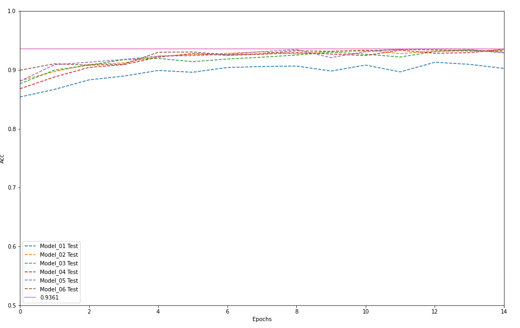
\includegraphics{Figures/figura_37.PNG}
\decoRule
\caption[Arquitectura modelo sustituto fashion-MNIST]{Exactitud de los modelos creados para el experimento.}
\label{fig:37}
\end{figure}

\subsection{Ataque de caja negra}
Se utiliza el conjunto de datos Fashion MNIST y utilizando los cinco modelos CNN víctimas con distintas arquitecturas, los cuales serán atacados. Todos obtuvieron una exactitud mayor al 90\% en los datos de validación. Por otro lado se creó un “modelo sustituto” el cual tiene por objetivo generar ejemplos adversarios utilizando la técnica de FGSM para ser usados en contra de los cinco modelos víctimas. En el modelo sustituto se crean los ejemplos adversarios indicados en las figuras ~\ref{fig:38} y ~\ref{fig:40} con distintos valores de $\varepsilon$. El caso $\varepsilon$= 0 corresponde a la imagen original, mayor a cero es una imagen adversaria. 

\begin{figure}[!h]
\centering
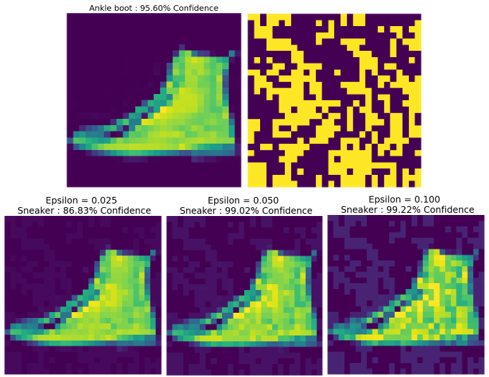
\includegraphics{Figures/figura_38.PNG}
\decoRule
\caption[Ataques adversarios en fashion MNIST.]{Ataques adversarios en fashion MNIST. Fila superior: A la izquierda la imagen original, derecha la matriz de dirección de perturbaciones
Fila inferior: Ejemplos adversarios a partir de distintos valores $\varepsilon$ y su resultado en modelo sustituto.}
\label{fig:38}
\end{figure}


\subsubsection{Preparación ataques adversarios}
Una vez entrenado el modelo sustituto se procedió a la creación del ejemplo adversario. Se implementó la técnica FGSM, en dónde utilizando el marco de trabajo Tensorflow se accedió a la función de gradiente descendiente con la cual pudimos saber donde realizar las modificaciones en la entrada para maximizar el error de clasificación.
Elegimos un par de imágenes de prueba para construir el ejemplo adversario. Se valida la imagen original en el modelo sustituto y este lo clasifica adecuadamente. Se obtiene la matriz de dirección de modificaciones que maximizan el error y luego se definieron distintos valores de $\varepsilon$, parámetro que determina el tamaño de las perturbaciones. 


\subsubsection{Primer ataque: Ankle boot}
En la figura~\ref{fig:38} la fila superior a la izquierda se encuentra la imagen original a utilizada en la creación de los ejemplos adversarios, a su derecha la matriz de dirección de perturbaciones y la fila inferior los ejemplos adversarios generados para distintos valores de $\varepsilon$ según se indica en su cabecera. La imagen original posee una clasificación de “Ankle boot” con un 95,6\% de confianza en el modelo sustituto, lo cual es correcto según su etiqueta. Las imágenes generadas con FGSM fueron clasificadas erróneamente, desde $\varepsilon$= 0.025 con una clasificación distinta en el modelo sustituto.


Ejecutamos el ataque sobre los modelos víctimas, obteniendo los resultados indicados en la figura~\ref{fig:39}. Podemos observar que en el caso de la imagen "Ankle boot" el ataque es 100\% efectivo en el modelo sustituto, éste afectó al 80\% de los modelos víctimas y en donde su ataque es efectivo a partir de un $\varepsilon$=0.1, en donde los modelos lo clasifican como "Coat", "Bag" y "Sneaker".

\begin{figure}[!h]
\centering
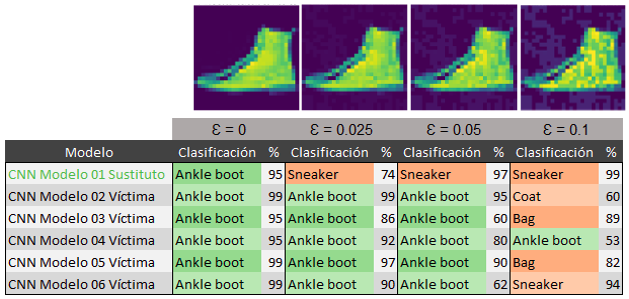
\includegraphics[scale = 0.90]{Figures/figura_39.PNG}
\decoRule
\caption[Resultados ataque 1 con fashion MNIST.]{Resultados ataque con fashion MNIST. En color verde se muestra para cada modelo y cada $\varepsilon$ las clasificaciones correctas. Este ejemplo adversario sólo logró su objetivo con un $\varepsilon$=0.1 en todos los modelos víctimas, a excepción del modelo 4. Fila superior la imagen asociada a cada $\varepsilon$.}
\label{fig:39}
\end{figure}



\subsubsection{Segundo ataque: Coat}
Se elige una segunda imagen del conjunto de datos de validación, cuya etiqueta lo cataloga como “Coat”. Se evalúa en el modelo sustituto y este lo clasifica correctamente con un 80.34\% de confianza, como se muestra en la primera fila, izquierda de la figura~\ref{fig:40}. Luego generamos los ejemplos adversarios de manera similar a como se hizo en el caso anterior con la “Ankle boot” y obtenemos las imágenes de la fila inferior de la figura~\ref{fig:40}.

Ejecutamos el ataque sobre los modelos víctimas, obteniendo los resultados indicados en la figura~\ref{fig:41}. Podemos observar que en el caso de la imagen Coat el ataque es 100\% efectivo en el modelo sustituto, éste afectó al 60\% de los modelos víctimas a partir de un $\varepsilon$=0.025 y luego a partir de un $\varepsilon$=0.05 afecta al 100\%, por lo que este ataque fue más efectivo que el “Ankle boot”, utilizando la misma técnica anterior solo variando la entrada seleccionada para la creación de los ejemplos adversarios.

\begin{figure}[!h]
\centering
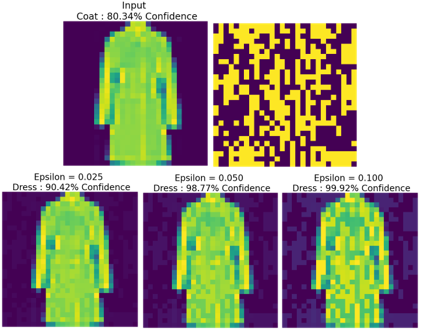
\includegraphics[scale = 1]{Figures/figura_40.PNG}
\decoRule
\caption[Resultados ataque 2 con fashion MNIST.]{Ataque adversario en Fashion MNIST. 
Fila superior: A la izquierda la imagen original, derecha la matriz de dirección de perturbaciones
Fila inferior: Ejemplos adversarios para distintos valores de $\varepsilon$ y su resultado en el modelo sustituto.
}
\label{fig:40}
\end{figure}


\begin{figure}[!h]
\centering
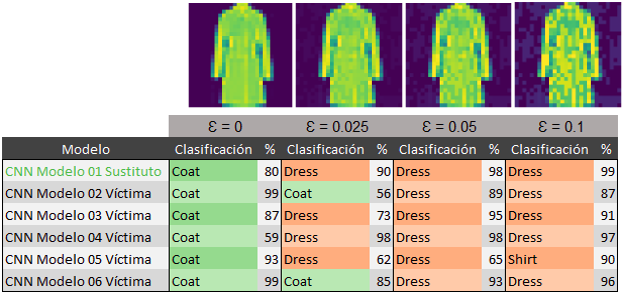
\includegraphics[scale = 0.85]{Figures/figura_41.PNG}
\decoRule
\caption[Resultados ataque 2 con fashion MNIST.]{Resultados ataque con fashion MNIST. En color verde se  muestra  para  cada  modelo  y  cada $\varepsilon$ las  clasificaciones  correctas. Este ejemplo adversario logró su objetivo con un $\varepsilon$=0.05 en todos los modelos víctimas. Fila superior la imagen asociada a cada $\varepsilon$}
\label{fig:41}
\end{figure}


La diferencia entre el primer y segundo ataque indica que la transferibilidad de los ejemplos adversarios depende de la entrada elegida, Por lo que el atacante debería crear varias entradas para su ataque y luego observar cual le servirá para su propósito.

En este experimento cada modelo poseía distintas cantidad de capas, neuronas, funciones de activación, algunas usan drop out y técnicas de aumento del conjunto de entrenamiento, otras no. Se comprueba la propiedad de transferibilidad de ejemplos adversarios generados en un modelo sustituto creado  para atacar a otros modelos a los cuales solo se accede como caja negra.



\subsubsection{Ataque con perturbaciones aleatorias}

Este experimento busca confirmar la efectividad de las técnicas que utilizan el gradiente descendiente para maximizar el error del clasificador de la redes profundas. Para ello realizaremos pruebas en donde se aplicarán perturbaciones a una imagen de entrada, pero en lugar de usar la matriz de dirección de modificaciones que entrega FGSM crearemos un conjunto de matrices con direcciones aleatorias. La figura~\ref{fig:42} muestra las perturbaciones creadas en el experimento, cada una de ellas fue aplicada a una imagen del conjunto de datos de validación para distintos valores de epsilon (tamaño de la perturbación).

En el ataque FGSM realizado sobre el modelo sustituto, cuyos resultados se encuentran en la figura~\ref{fig:39}, fue efectivo desde $\varepsilon$ 0.025. Los resultados del ataque aleatorio se encuentran en el anexo \ref{AppendixA}, en ellos se observa que en las 25 perturbaciones aleatorias, no se logró hacer fallar la clasificación de la misma imagen del modelo sustituto con $\varepsilon$ 0.05 como tampoco con 0.1, luego con 0.2 solo se logró el objetivo del ataque con una de las perturbaciones. Con $\varepsilon$ 0.5 se logró 100\% de efectividad del ataque, pero la imagen resultante no se consideraría un ejemplo adversario, ya que si bien logró el fallo en la clasificación de la imagen, la perturbación es perceptible para el ojo humano. La figura~\ref{fig:43} muestra una comparativa entre la imagen original (a la izquierda) utilizada en el ataque y los resultados de algunas de las perturbaciones aleatorias con  $\varepsilon$= 0.50.


\begin{figure}[!h]
\centering
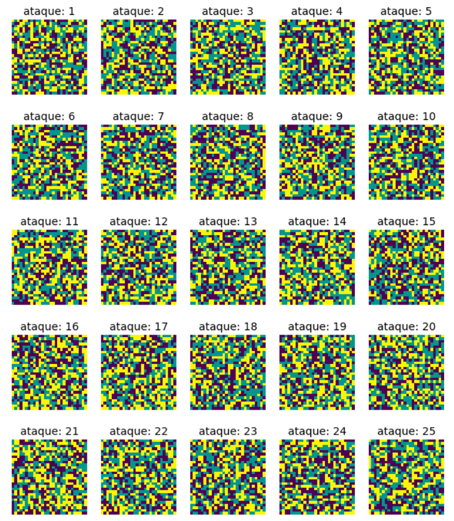
\includegraphics[scale = 1]{Figures/figura_42.PNG}
\decoRule
\caption[Matriz perturbaciones aleatorias aplicadas en el experimento con MNIST.]{Matriz de perturbaciones aleatorias aplicadas en el experimento.}
\label{fig:42}
\end{figure}

\begin{figure}[!h]
\centering
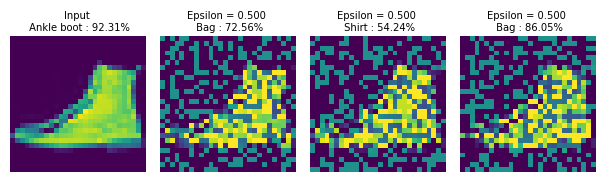
\includegraphics[scale = 0.85]{Figures/figura_43.PNG}
\decoRule
\caption[Matriz perturbaciones aleatorias aplicadas en el experimento con MNIST.]{Comparativa imagen original y perturbación aleatorias con $\varepsilon$=0.5}
\label{fig:43}
\end{figure}

La figura~\ref{fig:44} presenta una comparativa de porcentaje de efectividad de los ataques entre la técnica FGSM versus el ataque aleatorio.

\begin{figure}[!h]
\centering
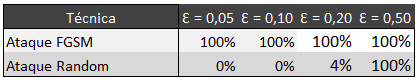
\includegraphics[scale = 1]{Figures/figura_44.PNG}
\decoRule
\caption[Comparativa de efectividad de los ataques FGSM y aleatorio.]{Comparativa de efectividad de los ataques}
\label{fig:44}
\end{figure}




\section{Ataque adversario en MobileNet V2 e ImageNet}
\subsection{Importación de red pre-entrenada}
Este experimento consistió en generar un ataque a una CNN de clasificación de imágenes con mayor cantidad de detalles, colores y formas, usando para ello un red pre-entrenada. Una red pre-entrenada es una red que fue entrenada previamente en un gran conjunto de datos, típicamente en una tarea de clasificación de imágenes a gran escala y que fue guardada. Esto permite contar con una arquitectura y eficacia ya probada. Por otro lado se atacó un modelo CNN que ha sido ampliamente utilizado, lo cual permitiría que las imágenes construidas para dicho propósito puedan ser utilizadas para atacar otros sistemas donde este se encuentre implementado. El modelo sobre el que se trabajó es el MobileNet V2 \parencite{r58} de la empresa Google. La arquitectura utiliza redes convolutivas con 32 filtros, seguidos de 19 capas residuales de cuello de botella y utiliza ReLU6 como función no lineal. Implementa kernel de tamaño 3x3 como también drop out y normalización durante el entrenamiento. El conjunto de datos utilizado es el ImageNet, el cual es un gran conjunto de datos que consta de imágenes 1.4 millones y 1000 clases cuyo propósito es el uso en investigación \parencite{r59}. 

\subsection{Preparación de ejemplos adversarios}

El conjunto de datos contiene una serie de objetos y animales en sus clases. En este experimento se trabajó con señaléticas de tránsito. La figura~\ref{fig:45}  muestra a las imágenes originales, clasificadas correctamente por el modelo. Estas imágenes no son parte del conjunto de datos, por lo que el modelo generaliza adecuadamente.

\begin{figure}[!h]
\centering
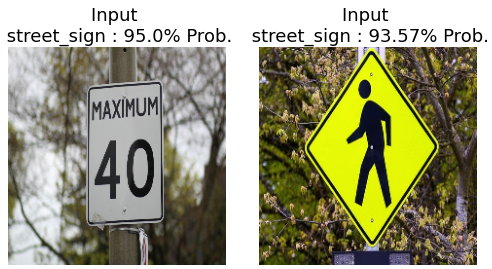
\includegraphics[scale = 1]{Figures/figura_45.PNG}
\decoRule
\caption[Ejemplo MobileNet V2 e ImageNet clasificación imágenes]{MobileNet V2 e ImageNet. Clasificador entrega correcta clasificación a las imágenes originales.}
\label{fig:45}
\end{figure}

Luego se procedió a la creación del ejemplo adversario, utilizando  la técnica de FGSM y las librerías Python 3 de Tensorflow. Con el marco de trabajo Tensorflow se obtiene la matriz de signos de gradientes para cada píxel de las imágenes, la cual indica en qué dirección modificar cada  imagen para maximizar su error en el clasificador (objetivo del ataque). La figura~\ref{fig:46} muestra como se ve dicha matriz al visualizarla como imagen respectivamente para las fotografías antes presentadas.

\begin{figure}[!h]
\centering
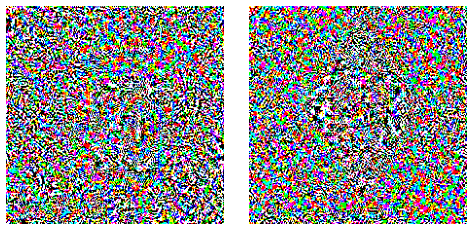
\includegraphics[scale = 1]{Figures/figura_46.PNG}
\decoRule
\caption[Ejemplo MobileNet V2 e ImageNet ataque FGSM]{Direcciones de las perturbaciones sugeridas en base a la gradiente descendiente para maximizar error. Izquierda: señalética velocidad máxima, derecha: Cruce peatonal.}
\label{fig:46}
\end{figure}

\subsubsection{Ataque señalética velocidad máxima 40}

Se crearon distintas imágenes, asociadas a distintos valores $\varepsilon$. A menor valor de $\varepsilon$, menos imperceptible el ataque a la vista humana, pero menor probabilidad de que el ataque sea efectivo. A mayor valor, más notable a la vista el ataque, aunque mayor probabilidad de hacer fallar la clasificación. La figura~\ref{fig:47} muestra los resultados de aplicación de perturbaciones para pequeños valores de $\varepsilon$, la primera imagen de la izquierda es la imagen original ($\varepsilon$ igual cero). Hacia la derecha van aumentando los valores de las perturbaciones. Con un pequeño $\varepsilon$=0.01 ya se logró engañar al clasificador, entregando una respuesta distinta a la original y siendo imperceptible la diferencia visual de ambas imágenes. 

\begin{figure}[!h]
\centering
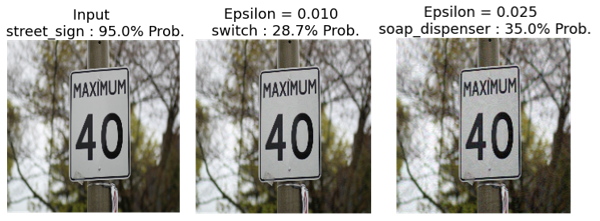
\includegraphics[scale = 0.85]{Figures/figura_47.PNG}
\decoRule
\caption[Perturbaciones FGSM con pequeños $\varepsilon$ señalética velocidad]{Perturbaciones FGSM con pequeños $\varepsilon$.}
\label{fig:47}
\end{figure}

A mayor valores de $\varepsilon$ observamos la notoriedad del ataque a la vista humana, y el modelo lo sigue clasificando erróneamente, como se muestra en la figura~\ref{fig:48}. Como se puede observar, un ataque adversario puede ser ejecutado fácilmente en un modelo importado. Esto permitiría al atacante crear localmente sus imágenes para luego utilizarlas atacando a otros clasificadores creados a partir de la importación del mismo modelo.

\begin{figure}[!h]
\centering
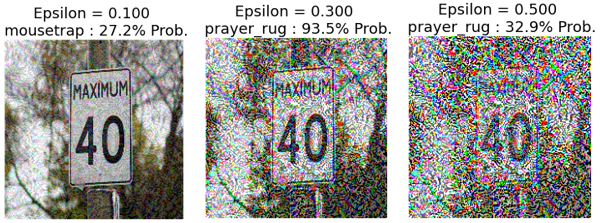
\includegraphics[scale = 0.80]{Figures/figura_48.PNG}
\decoRule
\caption[Perturbaciones FGSM con mayores $\varepsilon$ señalética velocidad]{Perturbaciones FGSM con $\varepsilon$ mayores.}
\label{fig:48}
\end{figure}


\subsubsection{Ataque señalética cruce peatonal}
El segundo ataque a señaléticas entregó similares resultados al anterior como se observa en las figuras~\ref{fig:49} y~\ref{fig:50}. con un pequeño $\varepsilon$=0.01 bastó para hacer fallar la clasificación y el resultado es imperceptible. Se puede observar en la figura~\ref{fig:50} con un $\varepsilon$=0.3 (imagen del centro) la probabilidad asignada a la clasificación errónea es incluso mayor a la entregada a la imagen original.

\begin{figure}[!h]
\centering
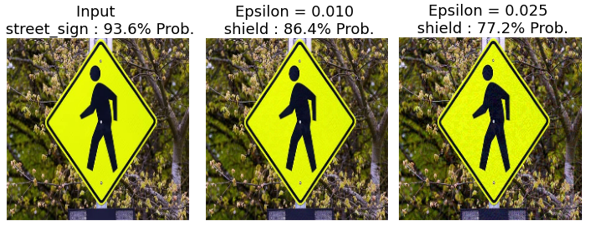
\includegraphics[scale = 0.85]{Figures/figura_49.PNG}
\decoRule
\caption[Perturbaciones FGSM con pequeños $\varepsilon$ en cruce peatonal]{Perturbaciones FGSM con pequeños $\varepsilon$.}
\label{fig:49}
\end{figure}

\begin{figure}[!h]
\centering
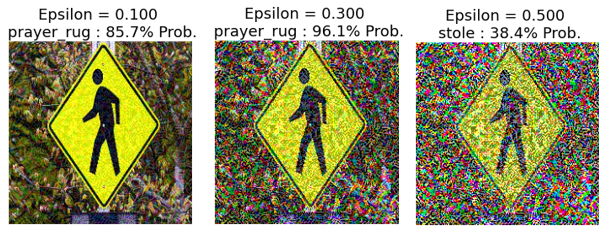
\includegraphics[scale = 0.83]{Figures/figura_50.PNG}
\decoRule
\caption[Perturbaciones FGSM con mayores $\varepsilon$ en cruce peatonal]{Perturbaciones FGSM con $\varepsilon$ mayores.}
\label{fig:50}
\end{figure}


\section{Ataque adversario placa de matrícula}

Este experimento tiene por propósito demostrar la vulnerabilidad que presentan los sistemas de reconocimiento automático de placas de matrículas de vehículos implementados en redes neuronales. Hoy en día existen varios software y hardware que ofrecen esta funcionalidad, cada día su uso se masifican más. Estos sistemas son utilizados por empresas de parking para controlar los accesos, autopistas para control de velocidad o cobro por uso de tramos, carros policiales para identificación automática de los vehículos que lo anteceden. Su arquitectura en general funciona de manera similar a la presentada en la figura~\ref{fig:51} que fue obtenida de una publicación \parencite{r60}. En la figura se observa que la entrada al sistema es la fotografía de vehículos,  en donde en primer lugar se detecta la presencia de coches, luego se identifica el área en donde se encuentra la matrícula en la imagen. El paso siguiente es rectificar la matrícula mejorando su ángulo, para posteriormente realizar el reconocimiento de los caracteres (OCR: Optical Character Recognition).

\begin{figure}[!h]
\centering
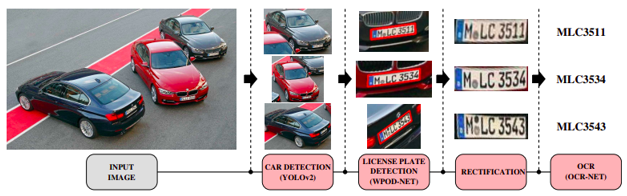
\includegraphics[scale = 0.90]{Figures/figura_51.PNG}
\decoRule
\caption[Flujo de operación de reconocimiento de placas matrículas]{Flujo de operación de reconocimiento de placas matrículas \parencite{r60}.}
\label{fig:51}
\end{figure}

La investigación tomada como referencia \parencite{r60} ofrece además los fuentes de su sistema de detección de matrícula, el cual se utilizó en este estudio como víctima de los ataques, provocando el fallo al clasificar los caracteres de las matrículas que fueron manipuladas.

\subsection{Sistema víctima}
Obtuvimos los fuentes del sistema propuesto en la investigación citada \parencite{r60} la cual divide su funcionamiento en los siguientes pasos:
\begin{enumerate}
    \item Detección de área de la matrícula:
        El sistema implementa un modelo pre-entrenado para la detección y extracción del área de las matrículas, llamado Wpod-Net. Este modelo es capaz de identificar matrículas de 10 países. La figura~\ref{fig:52} muestra los resultados que entrega esta red, enmarcando en rojo las placas matriculas detectadas en cada imagen. .
        
        \begin{figure}[!h]
        \centering
        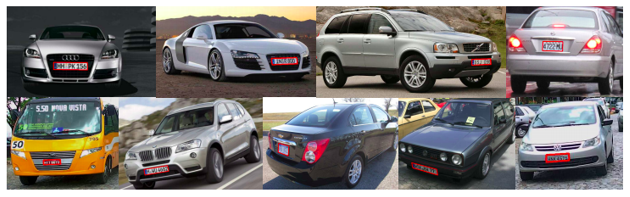
\includegraphics[scale = 0.9]{Figures/figura_52.PNG}
        \decoRule
        \caption[Detección de placas matrículas]{Detección de área de matrículas \parencite{r60}.}
        \label{fig:52}
        \end{figure}


    \item Identificación de espacio de caracteres:
        El sistema utiliza OpenCV para la segmentación de las áreas donde están ubicados los caracteres de la matrícula, de esta forma se prepara la información para el paso siguiente de reconocimiento de caracteres. La figura~\ref{fig:53} muestra los resultados de este proceso para una matrícula europea.

        \begin{figure}[!h]
        \centering
        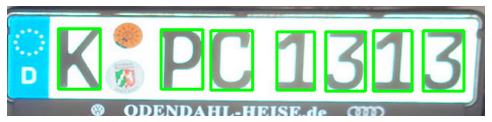
\includegraphics[scale = 1]{Figures/figura_53.PNG}
        \decoRule
        \caption[Identificación de espacio de caracteres en placas matrículas]{ Identificación de espacio de caracteres con OpenCV \parencite{r60}.}
        \label{fig:53}
        \end{figure}
    \item OCR [Optical Character Recognition]:
        Una vez detectada la ubicación de cada uno de los caracteres se itera uno a uno pasándolos a la entrada de una red convolutiva que determina su clase, permitiendo obtener la matrícula del coche. La figura~\ref{fig:54} muestra los resultados obtenidos en el artículo citado \parencite{r60}.

         \begin{figure}[!h]
        \centering
        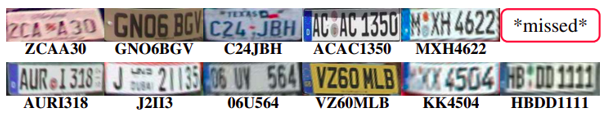
\includegraphics[scale = 0.85]{Figures/figura_54.PNG}
        \decoRule
        \caption[Resultados obtenidos del OCR]{ Resultados obtenidos del OCR \parencite{r60}.}
        \label{fig:54}
        \end{figure}
        
\end{enumerate}

\subsection{Pruebas previas al modelo: Imagen no perturbada}
Se descargó del repositorio Github el proyecto del artículo citado \parencite{r60}. El modelo del clasificado de caracteres posee un exactitud del 97.77\% en cual fue entrenado y validado con el conjunto de datos alfanumérico de 37.623 imágenes que posee 36 clases, aproximadamente 1.000 imágenes por cada caracter. El 10\% se utilizó para validación, y el restante 90\% en entrenamiento. La figura~\ref{fig:58} muestra los resultados del entrenamiento/validación del modelo.

 \begin{figure}[!h]
    \centering
    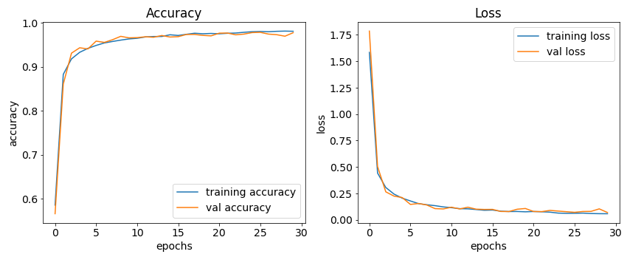
\includegraphics[scale = 0.85]{Figures/figura_58.PNG}
    \decoRule
    \caption[Resultados del entrenamiento/validación del clasificador de caracteres]{Resultados del entrenamiento/validación del modelo clasificador de caracteres alfanuméricos.}
    \label{fig:58}
\end{figure}



Ejecutamos la prueba con la imagen mostrada en la figura~\ref{fig:55}, observamos la correcta extracción de la matrícula.

 \begin{figure}[!h]
    \centering
    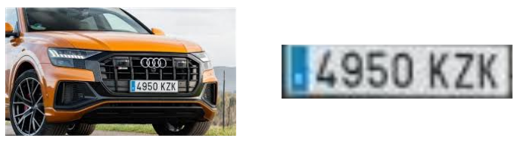
\includegraphics[scale = 1]{Figures/figura_55.PNG}
    \decoRule
    \caption[Pruebas preliminares, extracción de matrícula]{Pruebas preliminares, extracción de matrícula.}
    \label{fig:55}
\end{figure}

Luego continuamos el tratamiento de la imagen para facilitar la posterior lectura de los caracteres, como se muestra en la figura~\ref{fig:56}.

 \begin{figure}[!h]
    \centering
    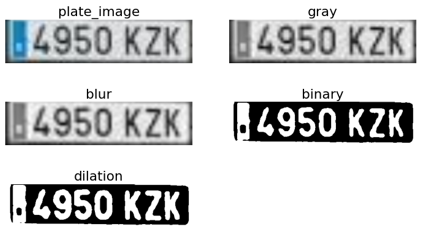
\includegraphics[scale = 1]{Figures/figura_56.PNG}
    \decoRule
    \caption[Pruebas preliminares, tratamiento de la imagen]{Pruebas preliminares, tratamiento de la imagen.}
    \label{fig:56}
\end{figure}

Posteriormente se identifica las áreas de los caracteres en la imagen como muestra la figura~\ref{fig:57}. Finalmente se procede con el reconocimiento de los caracteres.

 \begin{figure}[!h]
    \centering
    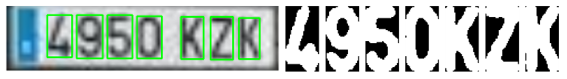
\includegraphics[scale = 0.85]{Figures/figura_57.PNG}
    \decoRule
    \caption[Pruebas preliminares, detección de área de caracteres en la imagen]{Pruebas preliminares, detección de área de caracteres en la imagen.}
    \label{fig:57}
\end{figure}


Los resultados de la clasificación de la imagen original (no perturbada) se encuentran en la figura~\ref{fig:59}, donde observamos que cada caracter fue correctamente identificado. Con esta prueba podemos confirmar que el modelo funciona y podemos comenzar con el ataque.

 \begin{figure}[!h]
    \centering
    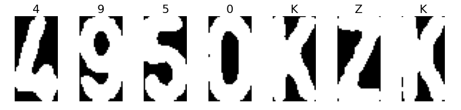
\includegraphics[scale = 1]{Figures/figura_59.PNG}
    \decoRule
    \caption[Pruebas preliminares, reconocimiento de los caracteres]{Pruebas preliminares, reconocimiento de los caracteres.}
    \label{fig:59}
\end{figure}

\subsection{Ataque adversario al modelo: Ataque físico}
En este experimento aplicaremos una técnica que simula un ataque físico (mundo real), es decir que simularemos aplicar una especie de parche a una placa matrícula con el objetivo que el clasificador de caracteres falle. Utilizaremos fuerza bruta, modificando un caracter hasta conseguir el objetivo. Se elige atacar utilizando el dígito “1” debido a que en la figura~\ref{fig:22} (ataque Jacobiano a MNIST de dígitos) se puede observar que es el número que menos perturbaciones requiere para hacer fallar al clasificador, por ende el que tiene mayor potencial.
Realizamos pruebas desde menos a más perturbaciones y se logra el objetivo, estableciendo el patrón de perturbación necesario para que el clasificador entregue una salida errónea.
El anexo \ref{AppendixB} muestra las perturbaciones realizadas a una placa matrícula alemana y a una placa matrícula española, de manera manual en un editor de imágenes, en donde se fueron colocando manchas  alrededor del dígito “1”, siguiendo algunas formas obtenidas de la figura~\ref{fig:22}. Se crearon 25 ejemplos adversarios para cada ataque, logrando con 6 obtener fallas en el clasificador en la placa matrícula alemana y 5 en la española.




\subsubsection{Ataque placa matrícula alemana}

La figura~\ref{fig:60} muestra las imágenes que lograron el objetivo del ataque con la placa matrícula alemana. En la interpretación del dígito 1 observamos ocasiones en que fue interpretado como el dígito 3, carácter T y E en el modelo víctima, lo que equivale al 24\% de efectividad del ataque. 

 \begin{figure}[!h]
    \centering
    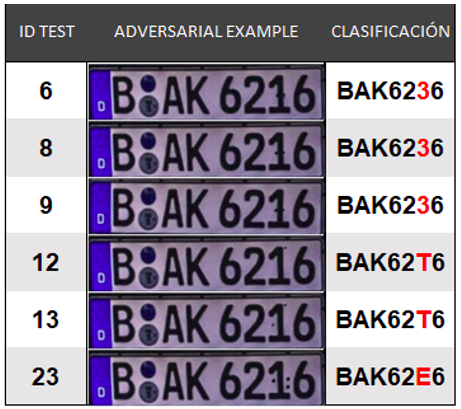
\includegraphics[scale = 1.1]{Figures/figura_60.PNG}
    \decoRule
    \caption[Ejemplos adversarios placa matrícula alemana]{Ejemplos adversarios que lograron hacer fallar al clasificador placa matrícula alemana.}
    \label{fig:60}
\end{figure}

Para comprobar que el ataque físico es efectivo, se imprimió una fotografía de uno de los ejemplos adversarios (id test 8 de figura~\ref{fig:60}) y luego esta imagen fue fotografiada y pasada nuevamente por el clasificador. La fotografía hizo fallar el modelo entregando el mismo resultado de la imagen modificada digitalmente. La figura~\ref{fig:61} muestra el ejemplo adversario impreso para efectuar el ataque físico, en donde el dígito “1” fue interpretado por un “3”. La alteración de la imagen es levemente perceptible.

 \begin{figure}[!h]
    \centering
    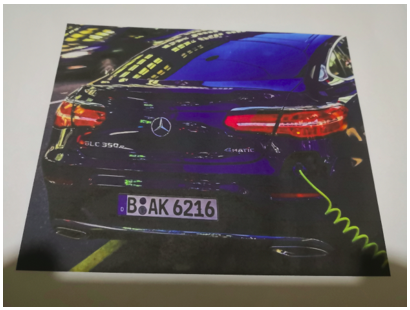
\includegraphics[scale = 1.1]{Figures/figura_61.PNG}
    \decoRule
    \caption[Ejemplo Adversario impreso matrícula alemana]{Ejemplo Adversario impreso. Modelo clasificó dígito “1” cómo “3”. Matrícula alemana.}
    \label{fig:61}
\end{figure}



\subsubsection{Ataque placa matrícula española}
La figura~\ref{fig:62} muestra las imágenes que lograron el objetivo del ataque de la placa matrícula española. Del total de 25 ejemplos adversarios, 5 lograron el fallo del clasificador en la interpretación del primer dígito 1 que posee la matrícula, donde dicho dígito fue interpretado como el carácter T en el modelo víctima. Esto equivale al 20\% de efectividad del ataque. El anexo \ref{AppendixB} posee la totalidad de pruebas realizadas.

 \begin{figure}[!h]
    \centering
    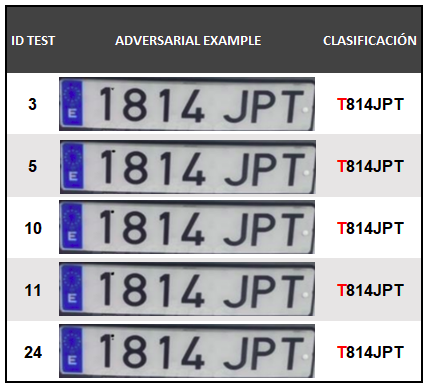
\includegraphics[scale = 1.1]{Figures/figura_62.PNG}
    \decoRule
    \caption[Resultados clasificador con una matrícula española]{Ejemplos adversarios que lograron hacer fallar al clasificador con una matrícula española.}
    \label{fig:62}
\end{figure}




\subsection{Defensa del modelo clasificador matrícula alemana}

Como se observa en los resultados del ataque, fue sencillo hacer fallar el modelo clasificador alfanumérico, esto puede tener relación a que la cantidad de datos de entrenamiento fue insuficiente, en comparación con el conjunto de datos MNIST de dígitos, el cual ofrece hasta 7 veces más imágenes por clase. Por otro lado, se realizan pruebas buscando una arquitectura de la red que ofrezca una robustez mayor frente al ataque. Por lo anterior se observan dos puntos de mejora:



\subsubsection{Defensa 1: Aumento del conjunto de entrenamiento}

El aumento del conjunto de entrenamiento es una técnica que permite aumentar las imágenes de entrenamiento a partir de las existentes, a través de funciones de zoom, rotaciones, desplazamientos, cambios de ángulos perspectivas, inversión vertical y horizontal. Si bien la versión original de la red implementó aumento del conjunto de entrenamiento, esta se modificó para hacerla más efectivo. Los resultados del ataque con la CNN original y la CNN con la nueva configuración se muestran en la figura~\ref{fig:63} en donde se logró reducir la efectividad del ataque del 24\% al 12\%. Entre las diferencias más destacables de esta nueva configuración, es que fue diseñada de acuerdo al formato de las imágenes de entrada, las cuales vienen centradas y sin rotación, por lo que se quitó la utilización de imágenes rotadas que traía el modelo original. Por otro lado se amplió la perspectiva (shear) de manera que generar más diversidad de muestras. El modelo original posee una exactitud del 97.77\%, mientras el modelo con la nueva configuración posee un 97.50\%, una leve disminución, pero a una mayor robustez.

 \begin{figure}[!h]
    \centering
    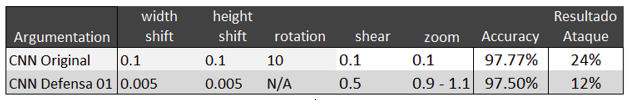
\includegraphics[scale = 0.85]{Figures/figura_63.PNG}
    \decoRule
    \caption[Resultados defensa 1]{Resultados defensa 1 y modelo original, ajuste al aumento del conjunto de entrenamiento.}
    \label{fig:63}
\end{figure}




\subsubsection{Defensa 2: Función de activación}

En el entrenamiento de redes neuronales se suele poner foco total en la exactitud y la pérdida del clasificador y en base a esto se evalúa si un modelo es bueno o no. En nuestro experimento, el modelo original presenta buenos indicadores, un 97.7\% de exactitud, sin embargo su robustez fue débil frente a unos pocos y simples ataques creados. Se experimentó modificando la arquitectura en búsqueda de mejorar la seguridad de la red frente a un ataque adversario. Estos cambios contemplan modificar cantidad de capas  y de neuronas de la red. La red en análisis es una CNN, de la cual nos enfocamos en cambios sobre las capas posteriores a las convulsiones.
El modelo original presenta a la salida de las convoluciones solo una capa oculta, con una función de activación de tipo RELU con drop out de 0.5 y 128 neuronas. El siguiente experimento consistió en mantener la arquitectura, solo cambiando la función de activación de la capa oculta por una SIGMOID cuya diferencia de observa en la figura~\ref{fig:64}.

 \begin{figure}[!h]
    \centering
    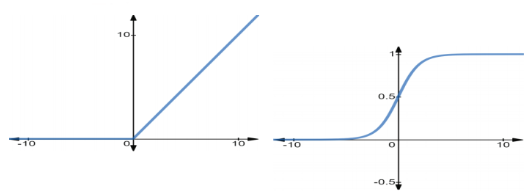
\includegraphics[scale = 1]{Figures/figura_64.PNG}
    \decoRule
    \caption[Función de activación]{Izquierda: Función de activación RELU. Derecha: SIGMOID \parencite{r62}.}
    \label{fig:64}
\end{figure}

Esta función posee mayor linealidad, lo cual podría generar fronteras distintas entre las clases de la red. Se utilizó como base la configuración mejorada de aumento del conjunto de entrenamiento. La exactitud de este nuevo modelo fue levemente mayor al original 97.79\% vs 97.77\%. La efectividad del ataque disminuyó, pasando del modelo original 24\% a  16\%, pero aumentó en un 4\% respecto a la defensa 1. Esto indica que si existe una relación entre la robustez y la función de activación del modelo.




\subsubsection{Defensa 3: Cambio arquitectura}

Se implementa una nueva arquitectura, pasando de una capa oculta a tres, con la siguiente distribución de neuronas en las capas ocultas: 512x512x1024, cada capa con drop out 0.5 y funciones de activación RELU->SIGMOID->SIGMOID. Se utilizó como base la configuración de la defensa 1. Este experimento logró ser totalmente robusto frente al ataque adversario del experimento, llevando la efectividad del ataque a 0\%. En cuanto a la exactitud, esta logró superar levemente a la del modelo original, 97.85\% vs 97.77\%. Esto comprueba la importancia de la arquitectura de un modelo y su estrategia de entrenamiento para brindar robustez frente a ataques.

También se probó con otras arquitecturas las cuales no mejoraron en gran medida la seguridad del modelo. La figura~\ref{fig:65} muestra los distintos resultados de los experimentos de defensa.

 \begin{figure}[!h]
    \centering
    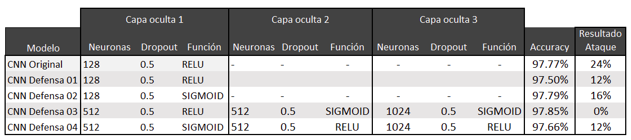
\includegraphics[scale = 0.85]{Figures/figura_65.PNG}
    \decoRule
    \caption[Resultados ataques en distintas arquitecturas. Matrícula alemana]{Resultados ataques en distintas arquitecturas. Matrícula alemana.}
    \label{fig:65}
\end{figure}




\subsection{Defensa del modelo clasificador matrícula española}

Se aplicó la mejor contramedida formulada para el ataque a la matrícula alemana para la defensa de la matrícula española, logrando replicar el resultado. La figura~\ref{fig:66} muestra los resultados en donde observamos que aplicando los cambios en el modelo señalado como “CNN Defensa 03” se logra evadir el 100\% de los ataques creados.
\begin{figure}[!h]
    \centering
    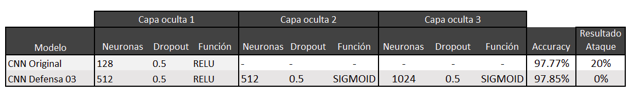
\includegraphics[scale = 0.85]{Figures/figura_66.PNG}
    \decoRule
    \caption[Resultados ataques en distintas arquitecturas. Matrícula española]{Resultados ataques en distintas arquitecturas. Matrícula española.}
    \label{fig:66}
\end{figure}